\documentclass[11pt]{article}  
\usepackage[margin=1in]{geometry}
\parindent=0in
\parskip=8pt
\usepackage{fancyhdr,amssymb,amsmath, graphicx, listings,float,subfig,enumerate,epstopdf,color,multirow,setspace,bm,textcomp}
\usepackage[usenames,dvipsnames]{xcolor}
\usepackage{hyperref}
\usepackage{graphicx}
\graphicspath{{./Images}}

\pagestyle{fancy}

\begin{document} 

\lhead{Assignment \#  \textcolor{red}{CHANGE ME!}}
\chead{Robert Denim Horton}
\rhead{\today}

\begin{center}\begin{Large}
CS 4720/5720 Design and Analysis of Algorithms

Homework \#  \textcolor{red}{CHANGE ME!}

Student: (Robert Denim Horton)
\end{Large}
\end{center}

\section*{Answers to homework problems:}

%\begin{center}
%	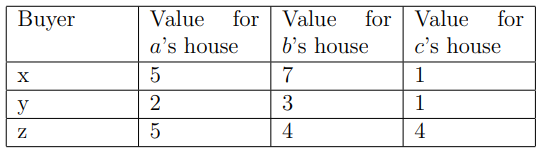
\includegraphics[scale=0.8]{Figure1.1}\\
%	Figure 1.1
%\end{center}

% Question 1
\begin{enumerate}
	\item QUESTION 1
		\begin{enumerate}[(a)]
		\item QUESTION 1 a)
		\item QUESTION 1 b)
	\end{enumerate}
\end{enumerate}
% Question 1 Answers
\textcolor{gray}{
Answers:
\begin{enumerate}
	\item ANSWER 1 \\
		\begin{enumerate}[(a)]
			\item ANSWER 1 a)\\
			Example of matrix in latex;\\
			\begin{center}
			 	$S(t)_{diag}=\begin{bmatrix} 
					S_1(t)  & 0.0 & 0.0 & 0.0 & 0.0 \\
					0.0  & S_2(2) & 0.0 & 0.0   & 0.0 \\
					0.0  & 0.0 & S_3(t) & 0.0 & 0.0 \\
					0.0  & 0 .0 & 0.0 & S_4(t) & 0.0 \\
					0.0  & 0 .0 & 0.0 & 0.0 & S_5(t) \\
				\end{bmatrix}$
			\end{center}
			\item ANSWER 1 b)\\
			How to use align with equations;\\
			\begin{align*}
				S(1) &=
					\begin{bmatrix} 
					0.01   &
					0.0 	&
					0.0 	&
					0.0 	&
					0.0 	&
					\end{bmatrix}
					 - 0.8 
					\begin{bmatrix} 
					0.99  & 0.0 & 0.0 & 0.0 & 0.0 \\
					0.0  & 1.0 & 0.0 & 0.0   & 0.0 \\
					0.0  & 0.0 & 1.0 & 0.0 & 0.0 \\
					0.0  & 0 .0 & 0.0 & 1.0 & 0.0 \\
					0.0  & 0 .0 & 0.0 & 0.0 & 1.0 \\
					\end{bmatrix}
			\end{align*}
		\end{enumerate}
\end{enumerate}
}

% Question 2
\begin{enumerate}
	\setcounter{enumi}{1}
	\item QUESTION 2
	\begin{enumerate}[(a)]
		\item QUESTION  2 A
		\item QUESTION  2 B  
	\end{enumerate}
\end{enumerate}
% Question 2 Answers
\textcolor{gray}{
Answers:
\begin{enumerate}
	\setcounter{enumi}{1}
	\item ANSWER  2 
	\begin{enumerate}[(a)]
		\item ANSWER  2 A
		\item ANSWER  2 B  
	\end{enumerate}
\end{enumerate}
}

% Question 3
\begin{enumerate}
	\setcounter{enumi}{1}
	\item QUESTION 3
	\begin{enumerate}[(a)]
		\item QUESTION  3 A
		\item QUESTION  3 B  
	\end{enumerate}
\end{enumerate}
% Question 3 Answers
\textcolor{gray}{
Answers:
\begin{enumerate}
	\setcounter{enumi}{1}
	\item ANSWER  3 
	\begin{enumerate}[(a)]
		\item ANSWER  3 A
		\item ANSWER  3 B  
	\end{enumerate}
\end{enumerate}
}

% Question 4
\begin{enumerate}
	\setcounter{enumi}{1}
	\item QUESTION 4
	\begin{enumerate}[(a)]
		\item QUESTION  4 A
		\item QUESTION  4 B  
	\end{enumerate}
\end{enumerate}
% Question 4 Answers
\textcolor{gray}{
Answers:
\begin{enumerate}
	\setcounter{enumi}{1}
	\item ANSWER  4 
	\begin{enumerate}[(a)]
		\item ANSWER  4 A
		\item ANSWER  4 B  
	\end{enumerate}
\end{enumerate}
}

% Question 5
\begin{enumerate}
	\setcounter{enumi}{1}
	\item QUESTION 5
	\begin{enumerate}[(a)]
		\item QUESTION  5 A
		\item QUESTION  5 B  
	\end{enumerate}
\end{enumerate}
% Question 5 Answers
\textcolor{gray}{
Answers:
\begin{enumerate}
	\setcounter{enumi}{1}
	\item ANSWER  5 
	\begin{enumerate}[(a)]
		\item ANSWER  5 A
		\item ANSWER  5 B  
	\end{enumerate}
\end{enumerate}
}
\end{document}
